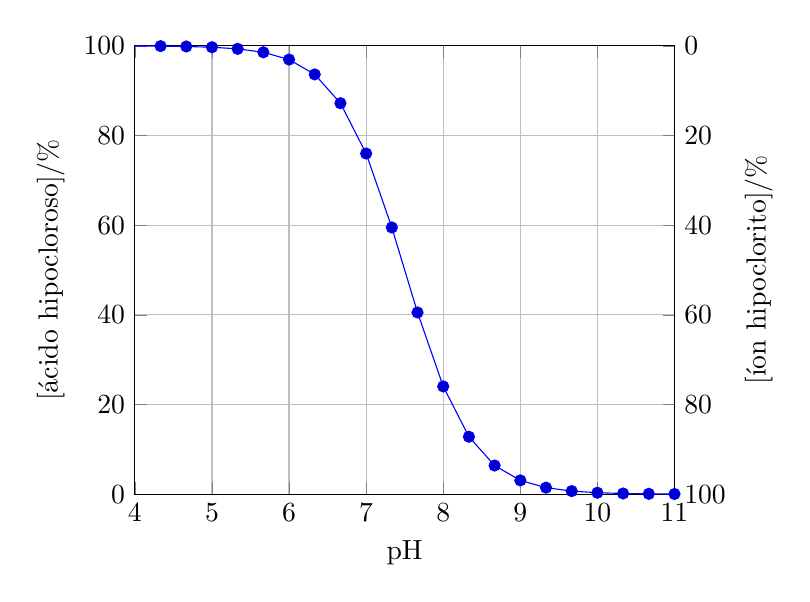
\begin{tikzpicture}
  \begin{axis}
    [
      y dir = reverse,
      axis y line* = right,
      ylabel = {[íon hipoclorito]/\%},
      axis x line  = none,
      xmin = 4, xmax = 11,
      ymin = 0, ymax = 100,
    ]
  \end{axis}
  \begin{axis}
    [
      grid = major,
      xlabel = {pH},
      ylabel = {[ácido hipocloroso]/\%},
      xmin = 4, xmax = 11,
      ymin = 0, ymax = 100,
      xtick = {4, 5, 6, 7, 8, 9, 10, 11},
    ]
    \addplot+ [domain=3:11]
    {
      100 * 10^(-x)/( 10^(-x) + 10^(-7.5) )
    };
  \end{axis}
\end{tikzpicture}
